\documentclass[a4paper,10pt]{article}
\usepackage[utf8]{inputenc}
\usepackage[spanish]{babel}
\usepackage[affil-it]{authblk}
\usepackage{enumerate}
\usepackage{graphicx}
\usepackage{hyperref}
\usepackage{amsmath}
\usepackage{amssymb}
\usepackage{cancel}
\usepackage[usenames, dvipsnames]{color}
\usepackage{tikz}
\usepackage[labelfont=bf]{caption}
\usepackage{subcaption} %Multiple images
\usepackage{multicol} % Multiple columns
\usepackage{float}
\usepackage{cleveref}
 \usepackage{relsize} % bigger math symbols
\usepackage[margin=1.4in]{geometry}
\usepackage[titletoc,toc,title]{appendix}
\usepackage{enumitem}
\usepackage{etoolbox}
\usetikzlibrary{calc}
\numberwithin{equation}{section}

% Circled words
\newcommand{\circled}[2][]{%
  \tikz[baseline=(char.base)]{%
    \node[shape = circle, draw, inner sep = 1pt]
    (char) {\phantom{\ifblank{#1}{#2}{#1}}};%
    \node at (char.center) {\makebox[0pt][c]{#2}};}}
\robustify{\circled}

%Appendices in spanish
\renewcommand{\appendixname}{Ap\'endices}
\renewcommand{\appendixtocname}{Ap\'endices}
\renewcommand{\appendixpagename}{Ap\'endices}

%Zero delimiter
\newcommand{\zerodel}{.\kern-\nulldelimiterspace}

%Columns separation
\setlength{\columnsep}{1cm}

%Indentation
\setlength{\parindent}{0ex}

%Multiple References

\crefrangelabelformat{equation}{(#3#1#4--#5\crefstripprefix{#1}{#2}#6)}

\usepackage{xparse}

%Boxes

\newcommand*{\boxcolor}{blue}
\makeatletter
\renewcommand{\boxed}[1]{\textcolor{\boxcolor}{%
\tikz[baseline={([yshift=-1ex]current bounding box.center)}] \node [rectangle, minimum width=1ex,rounded corners,draw] {\normalcolor\m@th$\displaystyle#1$};}}
 \makeatother

%Constantes
\newcommand{\euler}{\mathrm{e}}
\newcommand{\im}{i}

%Lemas, teoremas, definiciones y pruebas
\newcommand{\definicion}{\textbf{Definición: }}
\newcommand{\lema}{\textbf{Lema: }}
\newcommand{\teorema}{\textbf{Teorema: }}
\newcommand{\prueba}{\textbf{Prueba: }}
\newcommand{\proposicion}{\textbf{Proposición: }}
\newcommand{\corolario}{\textbf{Corolario: }}

% Definición de las secciones y su numeración

\makeatletter
\def\@seccntformat#1{%
  \expandafter\ifx\csname c@#1\endcsname\c@section\else
  \csname the#1\endcsname\quad
  \fi}
\makeatother

%opening
\title{Mecánica Clásica Tarea \# 14}
\author{Favio Vázquez\thanks{Correo: favio.vazquezp@gmail.com}}\affil{Instituto de Ciencias Nucleares. Universidad Nacional Autónoma de México.}
\date{}

\begin{document}

\makeatletter
\def\@maketitle{%
  \newpage
  \null
  \vskip 2em%
  \begin{center}%
  \let \footnote \thanks
    {\Large\bfseries \@title \par}%
    \vskip 1.5em%
    {\normalsize
      \lineskip .5em%
      \begin{tabular}[t]{c}%
        \@author
      \end{tabular}\par}%
    \vskip 1em%
    {\normalsize \@date}%
  \end{center}%
  \par
  \vskip 1.5em}
\makeatother

\maketitle

\section{Problema 1}

Utilizando únicamente la ecuación de la eikonal deduzca la ley de Snell.

\vspace{.3cm}

\underline{Solución:} \vspace{.3cm}

Recordemos la expresión para la ecuación de la eikonal,

\begin{equation}
 |\nabla S|^2(\mathbf{r}) = n^2(\mathbf{r}).
\end{equation}

Esta ecuación es simplemente el módulo de la ecuación de Huygens que puede 
escribirse como 

\begin{equation}
 \nabla S = n(\mathbf{r})\hat{\mathbf{s}},
\end{equation}

y también sabemos que el gradiente de esta ecuación define el vector de rayo de 
magnitud $|\mathbf{n}| = n$. Si ahora recordamos que la integración del gradiente 
sobre un camino cerrado se hace cero, tenemos que 

\begin{equation}
\oint_P \nabla S(\mathbf{r}) \cdot d\mathbf{r} = \oint_P \mathbf{n}(\mathbf{r}) 
\cdot d\mathbf{r} = 0.
\end{equation}

Consideremos ahora el caso en que el camino cerrado $P$ rodea una frontera que 
separa dos medios diferentes. Si hacemos que los lados del bucle perpendicular 
a la interfaz vayan a cero, entonces únicamente las partes de la integral de línea 
tangenciales al camino de la interfaz contribuirán en la misma. Ahora debido a que 
estas contribuciones deben sumar cero, las componentes tangenciales de los vectores 
de rato deben preservarse, esto es 

\begin{equation}
 (\mathbf{n} - \mathbf{n}') \times \hat{\mathbf{z}} = 0,
 \label{eq:preservacionTangencial}
\end{equation}

donde el primo se refiere al lado de la frontera al cual el rayo es transmitido, 
cuyo vector normal es $\hat{\mathbf{z}}$. Ahora imaginemos a un rayo atravesando 
la frontera y pasando a través de la región encerrada por el bucle de integración. 
Si $\theta$ y $\theta'$ son los ángulos de incidencia y transmisión, respectivamente, 
medidos desde la normal $\hat{\mathbf{z}}$ a través de la frontera, entonces la 
preservación de la componente tangencial del vector de rayo significa que, 
tomando en cuenta \eqref{eq:preservacionTangencial} y la definición del 
producto vectorial,

\begin{equation}
 \mathbf{n} \times \hat{\mathbf{z}} - \mathbf{n}' \times \hat{\mathbf{z}} = 0,
\end{equation}

\begin{equation}
 n\sen{\theta} - n'\sen{\theta'} = 0,
\end{equation}

esto debido a que $|\hat{\mathbf{z}}| = 1$, por lo tanto 

\begin{equation}
 \boxed{n\sen{\theta} = n'\sen{\theta'}.}
\end{equation}

Que es la ley de la refracción de Snell, descubierta primero por Ibn Sahl en 984 \cite{rashed}, 
y luego por Willebrod Snellius en 1621 \cite{holm}. Un análisis similar puede aplicarse al 
caso de los rayos reflejaos para mostrar que el ángulo de incidencia debe ser igual 
al ángulo de reflexión.

\section{Problema 2}

En el curso se mostró que la ecuación de la eikonal es una aproximación de onda 
pequeña de la ecuación de ondas. Encuentre ahora, a partir únicamente del principio 
de Fermat, las ecuaciones diferenciales que determinan los rayos de luz y la ecuación 
de la eikonal. Comente sobre la situación análoga entre las ecuaciones de movimiento 
de la mecánica y el principio de Hamilton.

\vspace{.3cm}

\underline{Solución:} \vspace{.3cm}

\section{Problema 3}

En el curso se demostró que la función principal de Hamilton es una solución completa 
de la ecuación de Hamilton-Jacobi correspondiente. ¿Será cierto el enunciado inverso 
de este, esto es, que una solución completa de la ecuación de Hamilton-Jacobi se puede 
ver como la función principal de Hamilton? Argumente su respuesta.

\vspace{.3cm}

\underline{Solución:} \vspace{.3cm}

\section{Problema 4}

Demuestre que un sistema es integrable sí y solo sí existen sistemas de coordenadas 
canónicas en las que la ecuación de Hamilton-Jacobi es totalmente separable.

\vspace{.3cm}

\underline{Solución:} \vspace{.3cm}

\section{Problema 5}

Reduzca a cuadraturas por el método de Liouville el ejemplo del péndulo esférico.

\vspace{.3cm}

\underline{Solución:} \vspace{.3cm}

Debajo se encuentra un diagrama del péndulo esférico,

\begin{figure}[H]
 \center 
 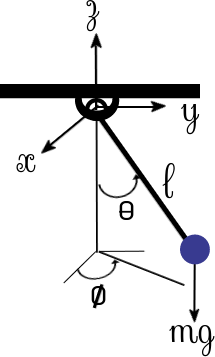
\includegraphics[scale=0.6]{problema5fig1}
 \caption{Péndulo esférico.}
 \label{fig:problema5fig1}
\end{figure}

recordamos que para el péndulo esférico la lagrangiana se escribe como 

\begin{equation}
 L = T - V = \frac{1}{2}ml^2(\dot{\theta}^2 + \dot{\phi}^2\sen^2{\theta} 
 - mgl\cos{\theta},
\end{equation}

podemos ahora escribir la hamiltoniana del sistema, primero obteniendo los momentos 
conjugados para las variables $\theta$ y $\phi$, 

\begin{equation}
 p_\theta = \frac{\partial L}{\partial \dot{\theta}} = ml^2\dot{\theta},
\end{equation}

\begin{equation}
 p_\phi = \frac{\partial L}{\partial \dot{\phi}} = ml^2\dot{\phi}\sen^2{\theta},
\end{equation}

de donde obtenemos 

\begin{equation}
 \dot{\theta} = \frac{p_\theta}{ml^2},
\end{equation}

y

\begin{equation}
 \dot{\phi} = \frac{p_\phi}{ml^2\sen^2{\theta}},
\end{equation}

y ahora utilizando 

\begin{equation}
 H = \sum_i p_i \dot{q}^2(q,p) - L, 
\end{equation}

la hamiltoniana del péndulo esférico resulta

\begin{equation}
 H = \frac{p_\theta^2}{2ml^2} + \frac{p_\phi^2}{2ml^2\sen^2{\theta}} 
 + mgl\cos{\theta}.
\end{equation}

Podemos notar ahora dos cosas. Primero, debido a que la coordenada $\phi$ es 
ignorable según la forma de la lagrangiana, entonces su momento conjugado se 
conservará, es decir que $p_\phi$ es constante, y además debido a que la energía 
cinética es una forma cuadrática de las velocidades y que la lagrangiana no depende 
explícitamente del tiempo, entonces la hamiltoniana es igual a la energía total 
del sistema, que también será una integral de movimiento. Usando la notación del
método de Liouville, podemos escribir esto de la siguiente forma 

\begin{equation}
  \frac{p_\theta^2}{2ml^2} + \frac{p_\phi^2}{2ml^2\sen^2{\theta}} 
 + mgl\cos{\theta} = I_1 = E,
 \label{eq:energiaPendEsf}
\end{equation}

\begin{equation}
 p_\phi = I_2.
 \label{eq:pphiPendEsf}
\end{equation}

Ahora hemos encontrado entonces dos integrales de movimiento, nos preguntamos ahora 
si están en involución, es decir si 

\begin{equation}
 \{I_1, I_2\} = 0,
\end{equation}

para ver esto recordamos la expresión para los paréntesis de Poisson, 

\begin{equation}
 \frac{\partial I_1}{\partial \theta}\cancelto{0}{\frac{I_2}{\partial p_\theta}} 
 - \frac{\partial I_1}{\partial p_\theta}\cancelto{0}{\frac{I_2}{\partial \theta}} + 
 \cancelto{0}{\frac{\partial I_1}{\partial \phi}}\frac{I_2}{\partial p_\phi} 
 - \frac{\partial I_1}{\partial p_\phi}\cancelto{0}{\frac{I_2}{\partial \phi}} = 
 0.
\end{equation}

Por lo tanto hemos demostrado que las dos integrales de movimiento que hemos encontrado 
están en involución, y debido a que hay tantas integrales de movimiento en involución como grados 
de libertad el sistema es integrable. Esto quiere decir que la uno forma $\omega = 
\sum_i p_idq^i$, que en términos de nuestras coordenadas y definiciones tiene la 
forma (despejando $p_\theta$ de \eqref{eq:energiaPendEsf}),

\begin{equation}
 \omega = \sqrt{2ml^2\left(I_1 - mgl\cos{\theta} - \frac{1}{2}\frac{I_2}{ml^2\sen^2{\theta}}
 \right)}d\theta + I_2d\phi,
\end{equation}

utilizando el teorema de Liouville es integrable, y al integrarla obtenemos 

\begin{equation}
 F = \int \sqrt{2ml^2\left(I_1 - mgl\cos{\theta} - \frac{1}{2}\frac{I_2}{ml^2\sen^2{\theta}}
 \right)}d\theta + I_2\phi.
\end{equation}

Y en vistas del mismo teorema podemos ver entonces a $F(q,I)$ como una función 
generadora de tipo dos, que al complementarla con 

\begin{equation}
 Q^i = \frac{\partial F(q,I)}{\partial I_i},
 \label{eq:QiPendEsf1}
\end{equation}

obtenemos una transformación canónica de coordenadas 

\begin{equation}
 (q,p) \leftrightarrow (Q,I),
\end{equation}

que nos lleva a un sistema canónico de coordenadas donde los impulsos son las 
integrales de movimiento. Ahora calculando las $Q^i$ utilizando \eqref{eq:QiPendEsf1}, 
obtenemos 

\begin{equation}
 Q^1 = \frac{\partial F}{\partial I_1} = \int \frac{ml^2}{\sqrt{2ml^2\left(I_1 -
 mgl\cos{\theta} - \frac{1}{2}\frac{I_2}{ml^2\sen^2{\theta}} \right)}}d\theta,
 \label{eq:Q1PendEsf1}
\end{equation}

\begin{equation}
 Q^2 = \phi - \int \frac{I_2}{\sen^2{\theta}\sqrt{2ml^2\left(I_1 - mgl\cos{\theta} - 
 \frac{1}{2}\frac{I_2}{ml^2\sen^2{\theta}} \right)}}d\theta.
 \label{eq:Q2PendEsf2}
\end{equation}

Y en nuestro nuevo sistema canónico $(Q^1,Q^2,I_1,I_2)$ tenemos 

\begin{equation}
 H = I_1 = E,
\end{equation}

por lo que 

\begin{equation}
 \dot{Q}^1 = \frac{\partial H}{\partial I_1} = 1,
\end{equation}

y 

\begin{equation}
 \dot{Q}^2 = \frac{\partial H}{\partial I_2} = 0.
\end{equation}

Y de estas ecuaciones podemos escribir, llamando a las constantes de integración 
$\beta^1$ y $\beta^2$ respectivamente, 

\begin{equation}
 Q^1 = t + \beta^1,
\end{equation}

\begin{equation}
 Q^2 = \beta^2,
\end{equation}

y utilizando estos resultados las ecuaciones \eqref{eq:Q1PendEsf1} y \eqref{eq:Q2PendEsf2}, 
quedan como 

\begin{equation}
 \boxed{t = -\beta^1 + \frac{\partial F}{\partial I_1} = \int \frac{ml^2}{\sqrt{2ml^2\left(I_1 -
 mgl\cos{\theta} - \frac{1}{2}\frac{I_2}{ml^2\sen^2{\theta}} \right)}}d\theta.}
\end{equation}

\begin{equation}
 \boxed{\phi = \beta^2 + \int \frac{I_2}{\sen^2{\theta}\sqrt{2ml^2\left(I_1 - mgl\cos{\theta} - 
 \frac{1}{2}\frac{I_2}{ml^2\sen^2{\theta}} \right)}}d\theta.}
\end{equation}

Con lo cual hemos reducido el péndulo esférico a cuadraturas utilizando el método 
de Liouville.

\begin{thebibliography}{10}
\bibitem{rashed}
R. Rashed, \emph{“Géométrie et dioptrique au Xe siècle: Ibn Sahl, 
Al-Quhi et Ibn Al-Haytham}, Las Belles Lettres, 1993.
\bibitem{holm}
D. Holm, \emph{Geometric Mechanics, Part I: Dynamics and Symmetry}, World Scientific, 
Imperial College Press, 2008.
\end{thebibliography}

\end{document}